%!TEX encoding=UTF-8 Unicode
%!TEX root=../tabarnac.tex

\def\len{6}
\def\wid{0.3}
\def\dis{0.1}

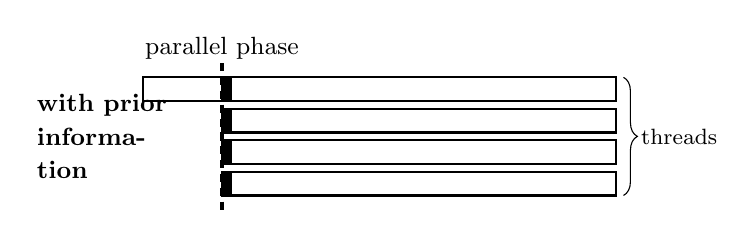
\begin{tikzpicture}
	\node[align=left, text width=1.7cm] at (-0.5,-\wid-1.5*\dis) (label1) {\bfseries\small with prior information};

	\draw[thick] (0,0)              rectangle +(\len, \wid);
	\draw[thick] (1,-\wid*0-\dis*1) rectangle +(\len-1,-\wid);
	\draw[thick] (1,-\wid*1-\dis*2) rectangle +(\len-1,-\wid);
	\draw[thick] (1,-\wid*2-\dis*3) rectangle +(\len-1,-\wid);

	\draw[fill=black] (1,0)              rectangle +(0.12,\wid);
	\draw[fill=black] (1,-\wid*0-\dis*1) rectangle +(0.12,-\wid);
	\draw[fill=black] (1,-\wid*1-\dis*2) rectangle +(0.12,-\wid);
	\draw[fill=black] (1,-\wid*2-\dis*3) rectangle +(0.12,-\wid);

	\draw[very thick,densely dashed] (1,1.6*\wid) -- +(0,-\wid*5-\dis*4.3) node[near start,pos=-0.1] {\small parallel phase};

	\draw [decorate,decoration={brace,amplitude=5pt}] (\len+.1,\wid) -- ++(0,-4*\wid-3*\dis) node [midway,right=1mm]{\footnotesize threads};

	% \draw (-1.35,-\wid*5) -- +(8.8,0); %separator


\end{tikzpicture}


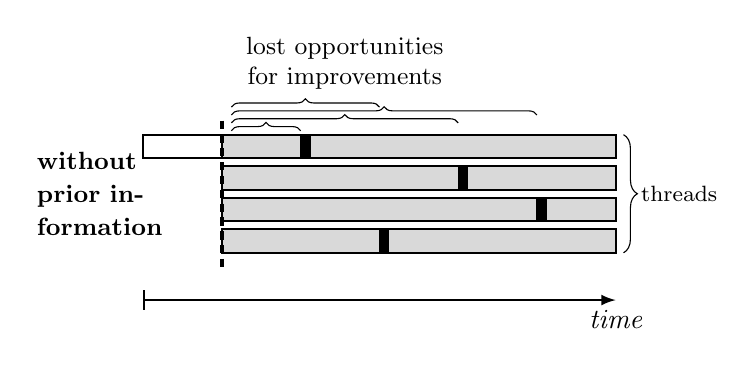
\begin{tikzpicture}
	\node[align=left, text width=2cm] at (-0.35,-\wid-1.5*\dis) (label1) {\bfseries\small without prior information};

	\draw[thick] (0,0)              rectangle +(\len, \wid);
	\draw[fill=gray!30, thick] (1,0)              rectangle +(\len-1, \wid);
	\draw[fill=gray!30, thick] (1,-\wid*0-\dis*1) rectangle +(\len-1,-\wid);
	\draw[fill=gray!30, thick] (1,-\wid*1-\dis*2) rectangle +(\len-1,-\wid);
	\draw[fill=gray!30, thick] (1,-\wid*2-\dis*3) rectangle +(\len-1,-\wid);

	\draw[fill=black] (2,0)              rectangle +(0.12,\wid);
	\draw[fill=black] (4,-\wid*0-\dis*1) rectangle +(0.12,-\wid);
	\draw[fill=black] (5,-\wid*1-\dis*2) rectangle +(0.12,-\wid);
	\draw[fill=black] (3,-\wid*2-\dis*3) rectangle +(0.12,-\wid);

	\draw[decorate,decoration={brace,amplitude=3pt}] (1+0.12,\wid+0.05) -- +(1-0.12,0);
	\draw[decorate,decoration={brace,amplitude=3pt}] (1+0.12,\wid+0.15) -- +(3-0.12,0)node[midway,above=3mm,align=center,font=\small] {\small lost opportunities\\ for improvements};
	\draw[decorate,decoration={brace,amplitude=3pt}] (1+0.12,\wid+0.25) -- +(4-0.12,0);
	\draw[decorate,decoration={brace,amplitude=3pt}] (1+0.12,\wid+0.35) -- +(2-0.12,0);

	\draw[very thick,densely dashed] (1,1.6*\wid) -- +(0,-\wid*5-\dis*4.3);

	\draw[decorate,decoration={brace,amplitude=5pt}] (\len+.1,\wid) -- ++(0,-4*\wid-3*\dis) node [midway,right=1mm]{\footnotesize threads};

	\draw[thick,|-latex] (0,-\wid*6) -- +(\len,0) node[below] {\itshape time};

\end{tikzpicture}
